\section{Vorgehensweise}\label{sec:vorgehensweise}

\subsection{Projektplan}\label{subsec:projektplan}

\subsubsection*{Übersicht}
\begin{figure}[h]
    \label{fig:projectPlan}
    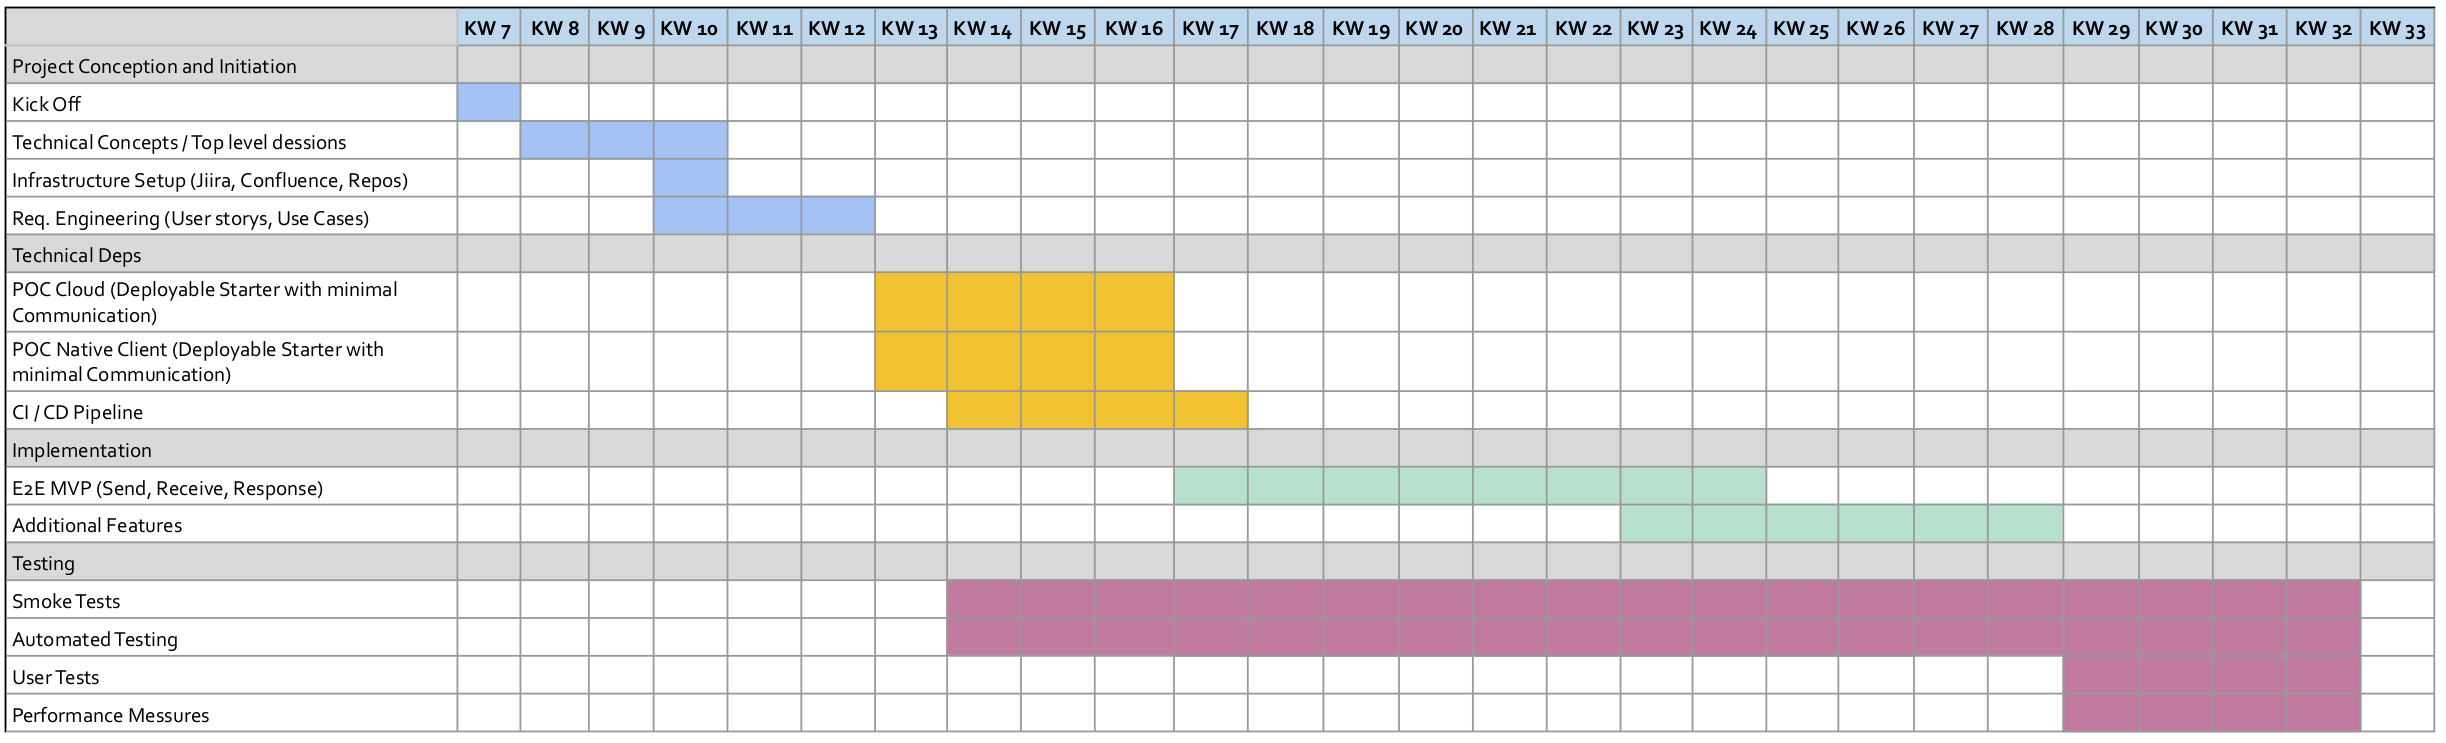
\includegraphics[width=\linewidth]{graphics/Projectplanning}\caption[Projektplan]{Projektplan}
\end{figure}

Das Projekt Cloudbasiertes Praxisrufsystem soll in vier Phasen umgesetzt werden.
Wobei sich diese Phasen teilweise überschneiden.

In der ersten Phase (KW7-KW13) soll die Infrastruktur die für das Projekt benötigt wird aufgebaut werden.
Es sollen Top Level Konzepte erfasst werden, wie das System funktionieren und kommunizieren soll.
Es sollen Technologien evaluiert werden, die zur Umsetzung verwendet werden können.
Es sollen die Prioriäteten und Wichtigsten Ziele des Projektes geklärt werden.
Diese Prioritäten und Ziele werden in Milestones festgehalten. (Siehe Kapitel XY).

In der zweiten Phase (KW13-KW17) soll ein Proof Of Concept erstellt werden.
Der die Recherchen und Konzepte aus Phase 1 verifiziert.
Wenn nötig werden hier Anpassungen an den gewählten Technologien gemacht.
Die Architektur und das Konzept werden weiter verfeinert.
Anforderungen werden konkretisiert.

In der dritten Phase (KW17-KW38) wird das Projekt schliesslich umgesetzt.
Zur Umsetzung gehört dabei vorzu die nächsten Anforderungen die Umzusetzen sind zu besprechen und die Konzepte dafür zu erweitern.
Als erster Teil soll dabei ein Minimal Viable Produkt erstellt werden.
Dieser MVP muss mit einem Backend kommunizieren können und Benachrichtigungen versenden und empfangen können.

Die vierte Phase (KW14-KW32) läuft parallel zur Dritten und beschäftigt sich mit dem Testing.
Automatisierte Unit und Smoke Tests sollen während der ganzen Projektdauer für die entwickelten Komponenten gemacht werden.
Zum Ende des Projekts soll das System zudem mit dem Benutzer getestet werden und auf Performance geprüft werden.

\clearpage
\subsection{Milestones}

In der Anfangsphase des Projektes wurden folgende Milestones definiert:

\begin{table}[h]
    \centering
    \begin{tabular}{|l|p{15cm}|}
        \hline
        \textbf{Id} & \textbf{Beschreibung}                                                                                                                                                                                         \\
        \hline
        M01         & Proof Of Concept - Setup. Ein Mobile Client kann auf IOS installiert werden und mit einem Backendservice kommunizieren. \\
        \hline
        M02         & Proof Of Concept - Messaging. Ein Mobile Client kann Benachrichtigungen empfangen und Push-Benachrichtigungen anzeigen. \\
        \hline
        M03         & Versenden mit Registration. Mobile Clients können sich beim Praxisrufsystem registrieren und Benachrichtungen empfangen. Alle registrierten Clients erhalten alle Benachrichtigungen. \\
        \hline
        M04         & Benachrichtigungen konfigurierbar. Der Mobile Client lädt seine Konfiguration vom Backend und zeigt dynamisch konfigurierte Buttons an über die Benachrichtigungen versendet werden.\\
        \hline
        M05         & Setup Wizard für Konfiguration. Ein Administrator kann das System über eine Benutzeroberfläche konfigurieren.  \\
        \hline
        M06         & 1:N Versenden Konfigurierbar. Es kann konfiguriert werden, welcher Client sich für welche Benachrichtigungen interessiert. Alle Clients erhalten nur für sie relevante Benachrichtigungen.  \\
        \hline
        M07         & Voice to Speech. Empfangene Benachrichtigungen können dem Benutzer vorgelesen werden. \\
        \hline
        M08         & Raspberry Pi Anbindung. Benachrichtigungen können über ein Raspberry Pi mit angeschlossenem Button versendet werden. \\
        \hline
        M09         & Sprachkommunikation 1:1. Der Mobile Client unterstützt direkte Anrufe zwischen zwei Geräten. \\
        \hline
        M10         & Sprachkommunikation 1:n. Der Mobile Client unterstützt Gruppenanrufe mit mehreren Geräten gleichzeitig. \\
        \hline
    \end{tabular}\label{tab:milestones}
\end{table}
\clearpage


